\chapter{Resultados y discusi\'on}
\label{ch:resultadosRadio}

El objetivo de este cap\'itulo (y de la segunda parte de esta tesis) es estimar el desempe\~no  de un detector de antenas de radio a la hora de detectar neutrinos ES.
Para ello, al igual que en Auger 

\section{C\'alculo de la exposici\'on}
	
	El c\'alculo de la exposici\'on se realiz\'o de manera similar a lo expuesto en la secci\'on \ref{sc:expoNu}, aunque existen ciertas diferencias, que se describen a continuaci\'on.
	%
	\begin{description}
	 \item[Inclusi\'on de la curvatura de la tierra] asd
	 
	 \begin{figure}[ht!]
		\centering
		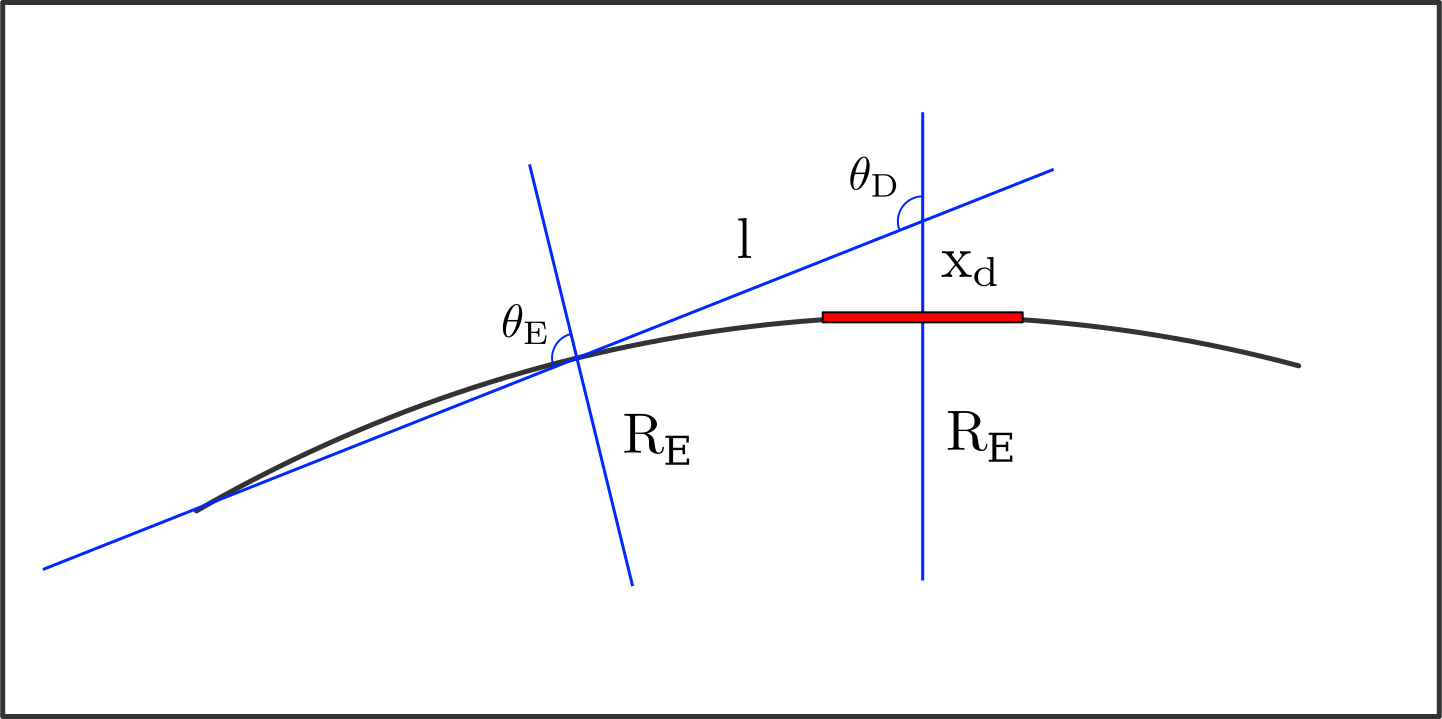
\includegraphics[width=0.8\textwidth]{./fig/appendix/curveEarthSketch.png}
		\caption{\label{fig:curveEarthSketch}
		Esquema del cambio en el angulo sobre el detector y el utilizado para calcular las probabilidades de interacci\'on del neutrino en la tierra.
		}
	\end{figure}
	 
	 \item[Manejo de la energ\'ia visible]
	 
	 \begin{figure}[h!]
		\begin{center}
			\includegraphics[width=0.9\textwidth]{fig/resultadosRadio/ev_etau}
			\caption{\label{fig:ev_etau} 
			Distribuci\'on de \ev{} dado \etau{} obtenida a partir de los decaimientos simulados con \tauola{}. 
			}
		\end{center}
	\end{figure}
	 
	 \item[Integraci\'on temporal y en superficie] Dado que esta parte de la tesis se enfoca en un detector gen\'erico, no ser\'a necesario realizar la integral por unidad de tiempo y \'area. 
	 Para analizar com cambia la exposici\'on en funci\'on de los distintos par\'ametros
	 La contribuci\'on de estos factores se obtendr\'a calculando la exposici\'on por unidad de \'area y tiempo, que luego podra ser multiplicada seg\'un 
	\end{description}
	%
	Teniendo en cuenta todos estos puntos, la ecuaci\'on para calcular la exposici\'on resulta:
	
	\begin{displaymath}
		\begin{aligned}
			{\cal E} (E_\nu) = 2 \pi T A
			\int_{0}^{\infty} 
			\int_{\theta_D^{cut}}^{\theta_D^{max}} 
			\int_{0}^{E_\nu} 
			\int_{0}^{E_\tau} 
			\epsilon (x_d,\theta_D,Ev) 
			\frac{e^{\frac{l(x_d)}{\lambda(E_\tau)}}}{\lambda(E_\tau)}\frac{dl(x_d)}{dx_d}
			P(E_v|E_\tau)\\
			P(E_\tau|E_\nu,\theta_E(\theta_D))
			\sin \theta_D \cos \theta_D
			dE_v dE_\tau  d\theta_D dx_d
		\end{aligned}
	\end{displaymath}
	
% 	\subsection{Manejo de la energ\'ia visible}
	
	
	\subsection{L\'imites de la t\'ecnica ES}
	\begin{figure}[h!]
		\begin{center}
			\includegraphics[width=0.9\textwidth]{fig/resultadosRadio/exposureFullEff_thetas}
			\caption{\label{fig:exposuresFluxThetas} Eventos esperados sobre el detector por unidad de \'area y tiempo, en funci\'on de la energ\'ia y suponiendo eficiencia m\'axima en el rango angular indicado.
			Naturalmente, la cantidad esperados aumenta a medida que lo hace el rango angular del \emph{detector ideal}.
			}
		\end{center}
	\end{figure}
	
	Integral en energ\'ia de las curvas de la figura \ref{fig:exposuresFluxThetas}
	
	\begin{figure}[h!]
		\begin{center}
			\includegraphics[width=0.9\textwidth]{fig/resultadosRadio/eventGain_thetas}
			\caption{\label{fig:gainThetas} Cantidad de eventos esperados como funci\'on del m\'aximo del rango angular, en relaci\'on al m\'aximo calculado ($N_{99.5}$).
			En rojo se observa un ajuste lineal de pendiente 0.127, que aproxima la curva para valores de $\theta_{MAX}>94$.
			Esto quiere decir que cada grado por encima de $94^\circ$ aporta un exceso de $\sim12.7\%$ eventos sobre el detector.
			}
			
		\end{center}
	\end{figure}
	
	
\section{C\'alculo de eficiencias}
	
	\begin{enumerate}
	 \item Especificar los bines a simular segun pesos de la lluvia.
	 \item Definir las caracteristicas del detector para calcular las eficiencias de disparo.
	 \item Determinar las eficiencias de identificaci\'on.
	\end{enumerate}

	
	\subsubsection{Pesos de las lluvias}

	\begin{figure}[ht!]
		\centering
		\begin{tabular}{cc}
		\includegraphics[width=0.45\textwidth]{fig/resultadosRadio/weights16_25.png} &
		\includegraphics[width=0.45\textwidth]{fig/resultadosRadio/weights16_75.png} \\
		\includegraphics[width=0.45\textwidth]{fig/resultadosRadio/weights17_25.png} &
		\includegraphics[width=0.45\textwidth]{fig/resultadosRadio/weights17_75.png} \\
		\includegraphics[width=0.45\textwidth]{fig/resultadosRadio/weights18_25.png} &
		\includegraphics[width=0.45\textwidth]{fig/resultadosRadio/weights18_75.png} \\
		\end{tabular}

		\caption{\label{fig:radioShWeights}
		Pesos de las lluvias en funci\'on de la altura de decaimiento y el \'angulo cenital para diferentes valores de energ\'ia visible, suponiendo un flujo $phi(E_\nu)\propto E^{-2}$ y eficiencia m\'axima.
		Estos gr\'aficos muestran la importancia relativa en la exposici\'on de los diferentes bines de energ\'ia visibles, \'angulos cenitales y alturas de decaimiento.
		Por ejemplo, para $\sim90^\circ$ y \cant{150}{m} se esperan del orden de 100 veces m\'as eventos a \cant{10^{17.25}}{eV} que a \cant{10^{18.25}}{eV}.
		}
	\end{figure}
	
	\subsubsection{Caracteristicas del detector}
	
	\subsubsection{Posibles topograf\'ias del detector}
	
	
	\textbf{Arreglo regular}
	
	\textbf{Arreglo tipo panal de abeja}
	
	\textbf{Arreglo tipo panal de abeja}
	
	Explicacion dle metodo.
	PLOT PAR DEFINIR TOPOGRAFIAS
	
	
	\begin{figure}[h!]
		\begin{center}
			\includegraphics[width=0.9\textwidth]{fig/resultadosRadio/17_00_89_90_00_00_00000_01238_60}
			\caption{asd}
			\label{fig:}
		\end{center}
	\end{figure}
	
	definicion del threshold
	
	descarte del canal muonico
	
% 	reescaleo por identificacion
	
	\begin{figure}[h!]
		\begin{center}
				\includegraphics[width=0.9\textwidth]{fig/resultadosRadio/eff75_0_4_0_1500_0_1500_0_60_0_1_0_17_0_m2.pdf} 
				\includegraphics[width=0.9\textwidth]{fig/resultadosRadio/eff75_0_4_0_1500_0_1500_0_60_0_1_0_17_5_m2.pdf}
				\includegraphics[width=0.9\textwidth]{fig/resultadosRadio/eff75_0_4_0_1500_0_1500_0_60_0_1_0_18_0_m2.pdf}
			\caption{asd}
			\label{fig:}
		\end{center}
	\end{figure}
	
	\begin{figure}[h!]
		\begin{center}
% 		\begin{ta
			\includegraphics[width=0.7\textwidth]{fig/resultadosRadio/CompRadioAuger_10_0_4_0_0_9_hc_modo1.pdf}
			\includegraphics[width=0.7\textwidth]{fig/resultadosRadio/CompRadioAuger_25_0_4_0_0_9_hc_modo1.pdf}
			\includegraphics[width=0.7\textwidth]{fig/resultadosRadio/CompRadioAuger_75_0_4_0_0_9_hc_modo1.pdf}
			\includegraphics[width=0.7\textwidth]{fig/resultadosRadio/CompRadioAuger_100_0_4_0_0_9_hc_modo1.pdf}
			\caption{asd}
			\label{fig:}
		\end{center}
	\end{figure}
	
	
	\subsection{Eficiencias de identificaci\'on - Discriminaci\'on en el fondo de eventos hadr\'onicos}
	\label{sc:identificacionRadio}

	Como se expuso en la primer parte de esta tesis, el mayor desaf\'io a la hora de detectar neutrinos ES mediante detectores de superficie resulta ser su discriminaci\'on en el fondo dominante de eventos hadr\'onicos.
	En Auger esto se logra debido a que los tanques \cher{} permiten detectar las lluvias j\'ovenes entre los eventos inclinados, a trav\'es de variables sensibles a la presencia de componente electromagn\'etica.
	En un detector de antenas de radio esta separaci\'on no resulta posible debido a que b\'asicamente toda la emisi\'on es generada en el m\'aximo de la lluvia por los electrones de media y baja energ\'ia.
	Sin embargo, su geometr\'ia permite salvar este escollo, ya que guarda informaci\'on sobre la ubicaci\'on en la que se produjo dicho m\'aximo.
	Para clarificar la situci\'on, en la figura \ref{fig:dg_vs_es_radio} se representa la emisi\'on \cher{} de un evento DG inclinado (un evento de background), y uno ES.
	%
	\begin{figure}[ht!]
		\centering
		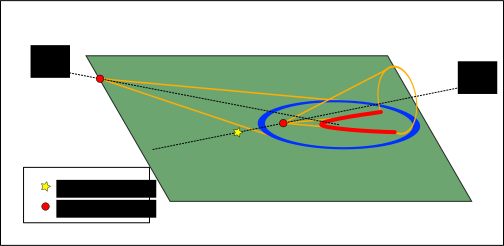
\includegraphics[width=\textwidth]{./fig/simulacionRadio/idRadio.png}
		\caption{\label{fig:dg_vs_es_radio}
		Esquema de las caracter\'isticas que permiten distinguir los eventos ES del fondo de lluvias hadr\'onicas horizontales (DG). Dado que las lluvias DG se inician alto en la atm\'osfera la apertura del cono \cher{} al nivel de la superficie (l\'inea azul) resulta mucho mayor que la que alcanzar\'ia en un evento ES, debido a que su m\'aximo se produce mucho m\'as cerca de la superficie.
	% 	Adem\'as de la apertura del cono, otro posible factor de discriminaci\'on puede ser la topograf\'ia de la se\~nal a nivel del suelo, ya que en los eventos DG imprimen elipses y los ES hip\'erbolas.
		}
	\end{figure}
	%
	La apertura del cono del evento DG a nivel del suelo resulta mayor que la que imprime el evento ES.
	Esto se debe a que los eventos hadr\'onicos inclinados se inician cerca del tope de la atm\'osfera, por lo que la emisi\'on debe recorrer hasta 36 atm\'osferas antes de alcanzar el detector.
	De esta manera, el cono \cher{} es cortado por el detector mucho m\'as lejos de su v\'ertice (que resulta ser aproximadamente el m\'aximo de la lluvia) que en eventos ES, los que se desarollan mucho m\'as cerca del detector.

	Para dar sustento a esta conjetura fue necesario simular eventos hadr\'onicos descendentes.
	Debido a 
	que se muestran en la figura \ref{fig:dg_thetas}.s

		\begin{figure}[ht!]
			\centering
			\begin{tabular}{cc}
			$85^\circ$ & $87^\circ$ \\
			\includegraphics[width=0.5\textwidth]{./fig/resultadosRadio/dg/{foorPrint_ZWv1.33_ntuples_v1.22_Downgoing_phi_90_19.5_85_90_100_1_E}.png} &
			\includegraphics[width=0.5\textwidth]{./fig/resultadosRadio/dg/{foorPrint_ZWv1.33_ntuples_v1.22_Downgoing_phi_90_18.5_87_90_100_2_E}.png}\\
			
			$88^\circ$ & $89^\circ$ \\
			\includegraphics[width=0.5\textwidth]{./fig/resultadosRadio/dg/{foorPrint_ZWv1.33_ntuples_v1.22_Downgoing_phi_90_18.5_89_90_100_5_E}.png} &
			\includegraphics[width=0.5\textwidth]{./fig/resultadosRadio/dg/{foorPrint_ZWv1.33_ntuples_v1.22_Downgoing_phi_90_19.5_89.5_90_100_3_E}.png}\\
			\end{tabular}
			\caption{\label{fig:dg_thetas}
			Huella sobre el detector
			}
		\end{figure}

	6800 horas cpu
	% 
	% 
	% Tambi\'en, se nota como la opograf\'ia de la huella en ambos casos es fundamentalmente distinta, ya que el evento DG imprime una elipse sobre el suelo y el evento ES una hip\'erbola.
	% En consecuencia se estudiar\'a si es posible explotar estas diferencias para identificar eventos ES.

	Por otra parte, en la figura 

	- eventos gigantes

	- se inician lejos y el campo cae como 1/R pero el drift es mayor debido a la baja densidad de la atm\'osfera

	- ver v4.20 en ntuple analizer mostrar que la velocidad sobre el eje y el ancho 

\subsubsection{Resumen del an\'alisis de la se\~nal}

	\begin{table}[ht!]
	\centering
	\begin{tabular}{|p{0.3\textwidth}|p{0.7\textwidth}|}
	\toprule
	Descripci\'on & Detalle \\
	\midrule\midrule
	Filtrado de la se\~nal & Respuesta plana en la banda \cant{30\text{-}80\text{/}120\text{-}900}{MHz} \\ \midrule
	Nivel de disparo local &  Entre \cant{25}{\frac{\mu V}{m}} y \cant{200}{\frac{\mu V}{m}} con un paso de \cant{25}{\frac{\mu V}{m}}\\ \midrule
	Disparo global & Antenas disparadas compatibles con un frente que se desplaza a la velocidad de la luz \\ \midrule
 	Nivel de identificaci\'on & Eficiencia entre 0.80 y 1.00 con un paso de 0.05 \\
	
	\bottomrule
	\end{tabular}
	\end{table}

	
\section{Desempe\~no de un detector de 100000 antenas}

El objetivo de esta secci\'on es discutir la posibilidad de armar un detector de 10000 antenas de radio cuyo fin ser\'ia detectar neutrinos ES.
Para ello, ser\'a necesario utilizar toda la informaci\'on racavada hasta el momento, as\'i como analizar las diferentes topolog\'ias con las que se podrian distribuir 


	\begin{figure}[h!]
		\begin{center}
			\includegraphics[width=\textwidth]{fig/resultadosRadio/limits_future}
			\caption{asd}
			\label{fig:}
		\end{center}
	\end{figure}